% Source-faithful schematic redraw of the cube and the named segments in printed question 18.
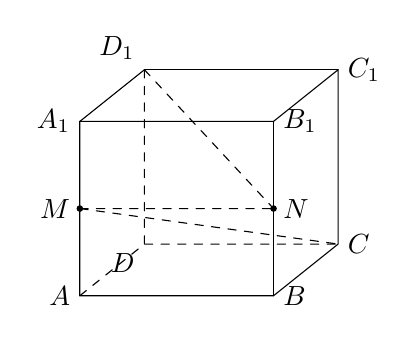
\begin{tikzpicture}[x=0.82cm,y=0.82cm,line cap=round,line join=round]
  \coordinate (A) at (0,0);
  \coordinate (B) at (3,0);
  \coordinate (C) at (4,0.8);
  \coordinate (D) at (1,0.8);
  \coordinate (Aone) at (0,2.7);
  \coordinate (Bone) at (3,2.7);
  \coordinate (Cone) at (4,3.5);
  \coordinate (Done) at (1,3.5);
  \coordinate (M) at (0,1.35);
  \coordinate (N) at (3,1.35);

  % Hidden cube edges as in the scanned schematic.
  \draw[dashed] (A)--(D) (D)--(C) (D)--(Done);
  % Visible cube edges.
  \draw (A)--(B)--(C)--(Cone)--(Bone)--(Aone)--cycle;
  \draw (Done)--(Cone);
  \draw (Aone)--(Done);
  \draw (A)--(Aone) (B)--(Bone);
  % The printed auxiliary segments and midpoint guide.
  \draw[dashed] (M)--(C) (M)--(N) (Done)--(N);
  \fill (M) circle (1.2pt) (N) circle (1.2pt);
  \node[left] at (A) {$A$};
  \node[right] at (B) {$B$};
  \node[right] at (C) {$C$};
  \node[below left] at (D) {$D$};
  \node[left] at (Aone) {$A_1$};
  \node[right] at (Bone) {$B_1$};
  \node[right] at (Cone) {$C_1$};
  \node[above left] at (Done) {$D_1$};
  \node[left] at (M) {$M$};
  \node[right] at (N) {$N$};
\end{tikzpicture}
